\chapter{Specifikacija programske potpore}
		
	\section{Funkcionalni zahtjevi}
			
			
			
			\noindent \textbf{Dionici:}
			
			\begin{packed_enum}
				
				\item Administrator
				\item Građanin
				\item Javni posjetitelj
				\item Razvojni tim
				\item Udruga za životinje
				\item Životinja 
				
			\end{packed_enum}
			
			\noindent \textbf{Aktori i njihovi funkcionalni zahtjevi:}
			
			
			\begin{packed_enum}
				\item  \underbar{Neregistrirani/neprijavljeni korisnik (inicijator) može:}
				
				\begin{packed_enum}
					
					\item Pristupiti naslovnoj stranici na kojoj može pregledati sve udruge
					\item Pristupiti detaljima profila udruge za životinje
					\begin{packed_enum}
						
						\item Dobiti uvid u profile pasa
						\item Dobiti uvid u statistike
						
					\end{packed_enum}
					\item Pristupiti rang listi
					\item Imati mogućnost registracije kao građanin ili udruga za životinje
					
				\end{packed_enum}
			
				\item  \underbar{Građani (inicijator) mogu:}
				
				\begin{packed_enum}
					
					\item Imati sve mogućnosti neprijavljenog/neregistiranog korisnika
					\item Prijaviti se u vlastiti profil
					\item Pregledati svoj raspored šetnji i svoje statistike šetnji
					\item Učiniti svoje statistike šetnji javnima
					\item Odabrati psa i željeni termin šetnje
					\item Preuzeti svoj raspored šetnji kao PDF 
					\item Mijenjati podatake o svom profilu
					
				\end{packed_enum}
			
				\item  \underbar{Udruge za životinje (inicijator) mogu:}
				
				\begin{packed_enum}
					
					\item Prijaviti se u vlastiti profil
					\item Mijenjati podatake o svom profilu
					\item Pristupiti naslovnoj stranici na kojoj može pregledati sve udruge
					\item Pristupiti profilima životinja i udruga za životinje
					
				\end{packed_enum}
			
				\item  \underbar{Administrator (inicijator) može:}
				
				\begin{packed_enum}
					
					\item Upravljati profilima građana, udruga i životinja
					\item Upravljati šetnjama
					
				\end{packed_enum}
			
				\item \underbar{Baza podataka (sudionik)}
				
					\begin{packed_enum}
						
						\item Dohvaćati podatke
						\item Pohranjivati podatke
						
					\end{packed_enum}
					
			
			\end{packed_enum}
			
			\eject 
			
			
				
			\subsection{Obrasci uporabe}
				
	
					
					\noindent \underbar{\textbf{UC1 - Registracija u sustav}}
					\begin{packed_item}
	
						\item \textbf{Glavni sudionik: } Javni posjetitelj
						\item  \textbf{Cilj:} Registracija u sustav kao građanin ili udruga za životinje
						\item  \textbf{Sudionici:} Baza podataka
						\item  \textbf{Preduvjet:} Korisničko ime i e-mail ne smiju biti već iskorišteni
						\item  \textbf{Opis osnovnog tijeka registracije udruge:}

						\item[] \begin{packed_enum}
							
							\item Odabir registracije udruge
							\item Unos korisničkog imena
							\item Unos e-mail adrese
							\item Unos lozinke
							\item Unos naziva udruge
							\item Unos broja telefona udruge
							\item Unos OIB-a udruge
							\item Unos adrese udruge
							\item Kliknuti gumb "Registracija"
							
							\end{packed_enum}
						
						\item  \textbf{Opis osnovnog tijeka registracije građanina:}
						
						\item[] \begin{packed_enum}
							
							\item Odabir registracije građanina
							\item Unos korisničkog imena
							\item Unos lozinke
							\item Unos imena
							\item Unos prezimena
							\item Unos e-mail adrese
							\item Unos broja telefona
							\item Kliknuti gumb "Registracija"
							
						\end{packed_enum}
					
						\item  \textbf{Opis mogućih odstupanja:}
					
						\item[] \begin{packed_item}
	
							\item[1.a] Korisničko ime već postoji u sustavu
							\item[] \begin{packed_enum}
								
								\item Sustav obavještava korisnika da unese drugo korinsičko ime
								\item Korisnik mijenja potrebne podatke te završava unos ili odustaje od registracije
								
								
								\end{packed_enum}
							\item[2.a] E-mail već postoji u sustavu
							\item[] \begin{packed_enum}
								
								\item Sustav obavještava korisnika da unese drugi e-mail
								\item Korisnik mijenja potrebne podatke te završava unos ili odustaje od registracije
								\end{packed_enum}
							
							
							\end{packed_item}
					\end{packed_item}
				
				\noindent \underbar{\textbf{UC2 - Prijava u sustav}}
					\begin{packed_item}
						
						\item \textbf{Glavni sudionik: } Građanin ili udruga
						\item  \textbf{Cilj:} Prijava u sustav kao građanin ili udruga
						\item  \textbf{Sudionici:} Baza podataka
						\item  \textbf{Preduvjet:} Građanin ili udruga moraju biti registrirani u sustav
						\item  \textbf{Opis osnovnog tijeka:}
						
						\item[] \begin{packed_enum}
							
							\item Unos korisničkog imena
							\item Unos lozinke
							\item Kliknuti gumb "Prijava"
						\end{packed_enum}
						
						\item  \textbf{Opis mogućih odstupanja:}
						
						\item[] \begin{packed_item}
							
							\item[1.a] Korisničko ime ne postoji u sustavu
							\item[] \begin{packed_enum}
								
								\item Sustav obavještava korisnika da je uneseno nepostojeće 
								korisničko ime
								\item Korisnik mijenja potrebne podatke te završava unos ili odustaje 
								od prijave
								
								
								
							\end{packed_enum}
							\item[2.a] Korisnik je unio krivu lozinku za navedeno korisničko ime
							\item[] \begin{packed_enum}
								
								\item Sustav obavještava korisnika da unese ispravnu lozinku
								\item Korisnik unosi ispravnu lozinku ili odustaje 
								od prijave
								
							\end{packed_enum}	
							
						\end{packed_item}
					\end{packed_item}
					
				\noindent \underbar{\textbf{UC3 - Pregled naslovne stranice}}
					\begin{packed_item}
						
						\item \textbf{Glavni sudionik: } Korisnik
						\item  \textbf{Cilj:} Pregled liste udruga
						\item  \textbf{Sudionici:} Baza podataka
						\item  \textbf{Preduvjet:} Pristup aplikaciji
						\item  \textbf{Opis osnovnog tijeka:} 
						
						\item[] \begin{packed_enum}
							
							\item Otvaranje aplikacije ili klik na gumb “Početna stranica”
							\item Pregled dostupnih podataka
						\end{packed_enum}
						
					\end{packed_item}
					
					\noindent \underbar{\textbf{UC3.1 - Pregled detalja udruga}}
					\begin{packed_item}
						
						\item \textbf{Glavni sudionik: } Korisnik
						\item  \textbf{Cilj:} Prikaz detalja udruga
						\item  \textbf{Sudionici:} Baza podataka
						\item  \textbf{Preduvjet:} -
						\item  \textbf{Opis osnovnog tijeka:} 
						
						\item[] \begin{packed_enum}
							
							\item Odabir željene udruge na naslovnoj stranici
							\item Prikaz podataka udruge
							\end{packed_enum}
						
					\end{packed_item}
					
				\noindent \underbar{\textbf{UC4 - Pretraživanje udruga}}
					\begin{packed_item}
						
						\item \textbf{Glavni sudionik: } Korisnik
						\item  \textbf{Cilj:} Pronaći udrugu preko upisa imena ili lokacije
						\item  \textbf{Sudionici:} Baza podataka
						\item  \textbf{Preduvjet:} -
						\item  \textbf{Opis osnovnog tijeka:} 
						
						\item[] \begin{packed_enum}
							
							\item Odabrati gumb "Pretraživanje" i upisati u polje za pretraživanje
							\item Odabrati željenu udrugu
							\end{packed_enum}
						
					\end{packed_item}
				
					\noindent \underbar{\textbf{UC5 - Prijava šetnje}}
					\begin{packed_item}
						
						\item \textbf{Glavni sudionik: } Građanin
						\item  \textbf{Cilj:} Prijaviti šetnju sa željenom životinjom i željenim terminom
						\item  \textbf{Sudionici:} Životinje, Baza podataka
						\item  \textbf{Preduvjet:} Prijavljen u sustav
						\item  \textbf{Opis osnovnog tijeka:}
						
						\item[] \begin{packed_enum}
							
							\item Odabire se željeni termin i duljina šetnju
							\item Odaberu se svi željeni psi za šetnju koji su slobodni u odabranom terminu te koji odgovaraju vrsti šetnje
							\item Odabire se opcija “Prijavi šetnju”
							\item Pokaže se stranica s pregledom podataka o šetnji
							\item Potvrda šetnje
							
						\end{packed_enum}
						
						\item  \textbf{Opis mogućih odstupanja:}
						
						\item[] \begin{packed_item}
							
							\item[1.a] Građanin se u odabranom terminu već prijavio za drugu šetnju
							\item[] \begin{packed_enum}
								
								\item Sustav obavještava korisnika da je u željenom terminu već zauzet te zatraži od njega promjenu termina
								\item Građanin mijenja termin ili odustaje od šetnje
								
								
							\end{packed_enum}
							\item[5.a] Nema slobodnih pasa u odabranom terminu
							\item[] \begin{packed_enum}
								
								\item Nakon potvrde šetnje, sustav obavještava korisnika da su odabrani psi već zauzeti u željenom terminu
							\end{packed_enum}
							
							
						\end{packed_item}
					\end{packed_item}
					
				\noindent \underbar{\textbf{UC6 - Pregled vlastitog rasporeda}}
					\begin{packed_item}
	
						\item \textbf{Glavni sudionik: }Građanin
						\item  \textbf{Cilj:} Pregledati vlastiti raspored šetnji
						\item  \textbf{Sudionici:} Baza podataka
						\item  \textbf{Preduvjet:} Korisnik je prijavljen u sustav
						\item  \textbf{Opis osnovnog tijeka:}

						\item[] \begin{packed_enum}
	
							\item Odabire se opcija “Raspored”
							\item Prikaz vlastitog rasporeda
							\end{packed_enum}
							
						\item  \textbf{Opis mogućih odstupanja: -}
						\end{packed_item}
							
							
				\noindent \underbar{\textbf{UC6.1 - Preuzimanje vlastitog rasporeda}}
					\begin{packed_item}
						
						\item \textbf{Glavni sudionik: }Građanin
						\item  \textbf{Cilj:} Preuzeti svoj raspored šetnji
						\item  \textbf{Sudionici:}  Životinja, Baza podataka
						\item  \textbf{Preduvjet:} Korisnik je prijavljen u sustav
						\item  \textbf{Opis osnovnog tijeka:}
						
						\item[] \begin{packed_enum}
							
							\item Na vlastitom profilu otvori se raspored
							\item Odabire se početni i završni datum za raspored koji se želi preuzeti
							\item Klikne se “Preuzmi raspored”
						
							\end{packed_enum}
				
						\item  \textbf{Opis mogućih odstupanja: -}
		
						\end{packed_item}
								
								
				\noindent \underbar{\textbf{UC7 - Pregled osobnih podataka}}
					\begin{packed_item}
							
						\item \textbf{Glavni sudionik: }Građanin, Udruga
						\item  \textbf{Cilj:} Pregled osobnih podataka koji su zapisani u sustavu
						\item  \textbf{Sudionici:} Baza podataka
						\item  \textbf{Preduvjet:} Korisnik je prijavljen u sustav
						\item  \textbf{Opis osnovnog tijeka:}
						
						\item[] \begin{packed_enum}
							
							\item Građanin ili Udruga odabiru opciju “Profil”
							\item Prikazuju se osobni podaci
							\end{packed_enum}
						
						\item  \textbf{Opis mogućih odstupanja: -}
						\end{packed_item}
							
							
				\noindent \underbar{\textbf{UC7.1 - Promjena osobnih podataka}}
					\begin{packed_item}
						
						\item \textbf{Glavni sudionik: }Udruga, Građanin
						\item  \textbf{Cilj:} Promjena osobnih podataka na nove ili ispravne vrijednosti
						\item  \textbf{Sudionici:} Baza podataka
						\item  \textbf{Preduvjet:} Korisnik je prijavljen u sustav
						\item  \textbf{Opis osnovnog tijeka:}
						
						\item[] \begin{packed_enum}
						
							\item Građanin ili Udruga pregledavaju svoje podatke
							\item Odabire se opcija “Uredi podatke”
							\item Korisnik uredi podatke
							\item Odabirom opcije “Spremi podatke” se spremaju podaci
							\end{packed_enum}
						
						\item  \textbf{Opis mogućih odstupanja:}
						
						\item[] \begin{packed_item}
						
							\item[4.a] Podaci nisu ispravni
							\item[] \begin{packed_enum}
								
								\item Sustav prepoznaje neispravne podatke te zatraži njihov ispravak
							
								\end{packed_enum}


							\end{packed_item}
						\end{packed_item}
					
					\noindent \underbar{\textbf{UC8 - Pristup statistici}}
					\begin{packed_item}
						
						\item \textbf{Glavni sudionik: }Korisnik
						\item  \textbf{Cilj:} Pregled rang liste šetača
						\item  \textbf{Sudionici:} Baza podataka
						\item  \textbf{Preduvjet:} -
						\item  \textbf{Opis osnovnog tijeka:}
						
						\item[] \begin{packed_enum}
							
							\item Odabire se opcija “Statistika”
							\item Prikaže se statistika svih šetnji te rang liste
						\end{packed_enum}
						
						\item  \textbf{Opis mogućih odstupanja: -}
					\end{packed_item}
				
				\noindent \underbar{\textbf{UC9 - Pregled vlastitih statistika šetnji}}
				\begin{packed_item}
					
					\item \textbf{Glavni sudionik: }Građanin
					\item  \textbf{Cilj:} Pregled vlastitih statistika šetnji i mogućnost odabira šetnje kao javne
					\item  \textbf{Sudionici:} Baza podataka
					\item  \textbf{Preduvjet:} Prijavljen u sustav
					\item  \textbf{Opis osnovnog tijeka:}
					
					\item[] \begin{packed_enum}
						
						\item Na vlastitom profilu otvori se statistika šetnji
						\item Odabirom opcije "Uredi podatke" za statistiku se može se postaviti je li javna ili privatna
					\end{packed_enum}
					
					\item  \textbf{Opis mogućih odstupanja: -}
					
				\end{packed_item}
			
			\noindent \underbar{\textbf{UC10 - Pregled profila životinja}}
			\begin{packed_item}
				
				\item \textbf{Glavni sudionik: }Korisnik
				\item  \textbf{Cilj:} Pregled podataka za pojedinu životinju
				\item  \textbf{Sudionici:} Životinja, Baza podataka
				\item  \textbf{Preduvjet:} -
				\item  \textbf{Opis osnovnog tijeka:}
				
				\item[] \begin{packed_enum}
					
					\item Odabire se udruga čije se životinje žele pregledati
					\item Prikazuju se podaci životinja
					
				\end{packed_enum}
				
				\item  \textbf{Opis mogućih odstupanja: -}
			\end{packed_item}
			
			\noindent \underbar{\textbf{UC10.1 - Dodavanje i brisanje životinja}}
			\begin{packed_item}
				
				\item \textbf{Glavni sudionik: }Udruga
				\item  \textbf{Cilj:} Dodavanje i brisanje životinja u sustavu
				\item  \textbf{Sudionici:} Životinja, Baza podataka
				\item  \textbf{Preduvjet:} Korisnik je prijavljen u sustav kao udruga
				\item  \textbf{Opis osnovnog tijeka:}
				
				\item[] \begin{packed_enum}
					
					
					\item Odabire se opcija "Uredi pse" na vlastitom profilu udruge
					\item Odabirom opcije "Izbriši životinju" pored odabrane životinje ona se briše iz sustava
					\item Odabirom opcije "Dodaj psa" otvara se forma za popunjavanje podataka o novom psu te, klikom na gumb "Dodaj", on se dodaje u sustav
					
				\end{packed_enum}
				
				\item  \textbf{Opis mogućih odstupanja: }Podaci se nisu uspješno spremili
			\end{packed_item}
		
				\eject
				\subsubsection{Dijagrami obrazaca uporabe}
					
					\begin{figure}[H]
						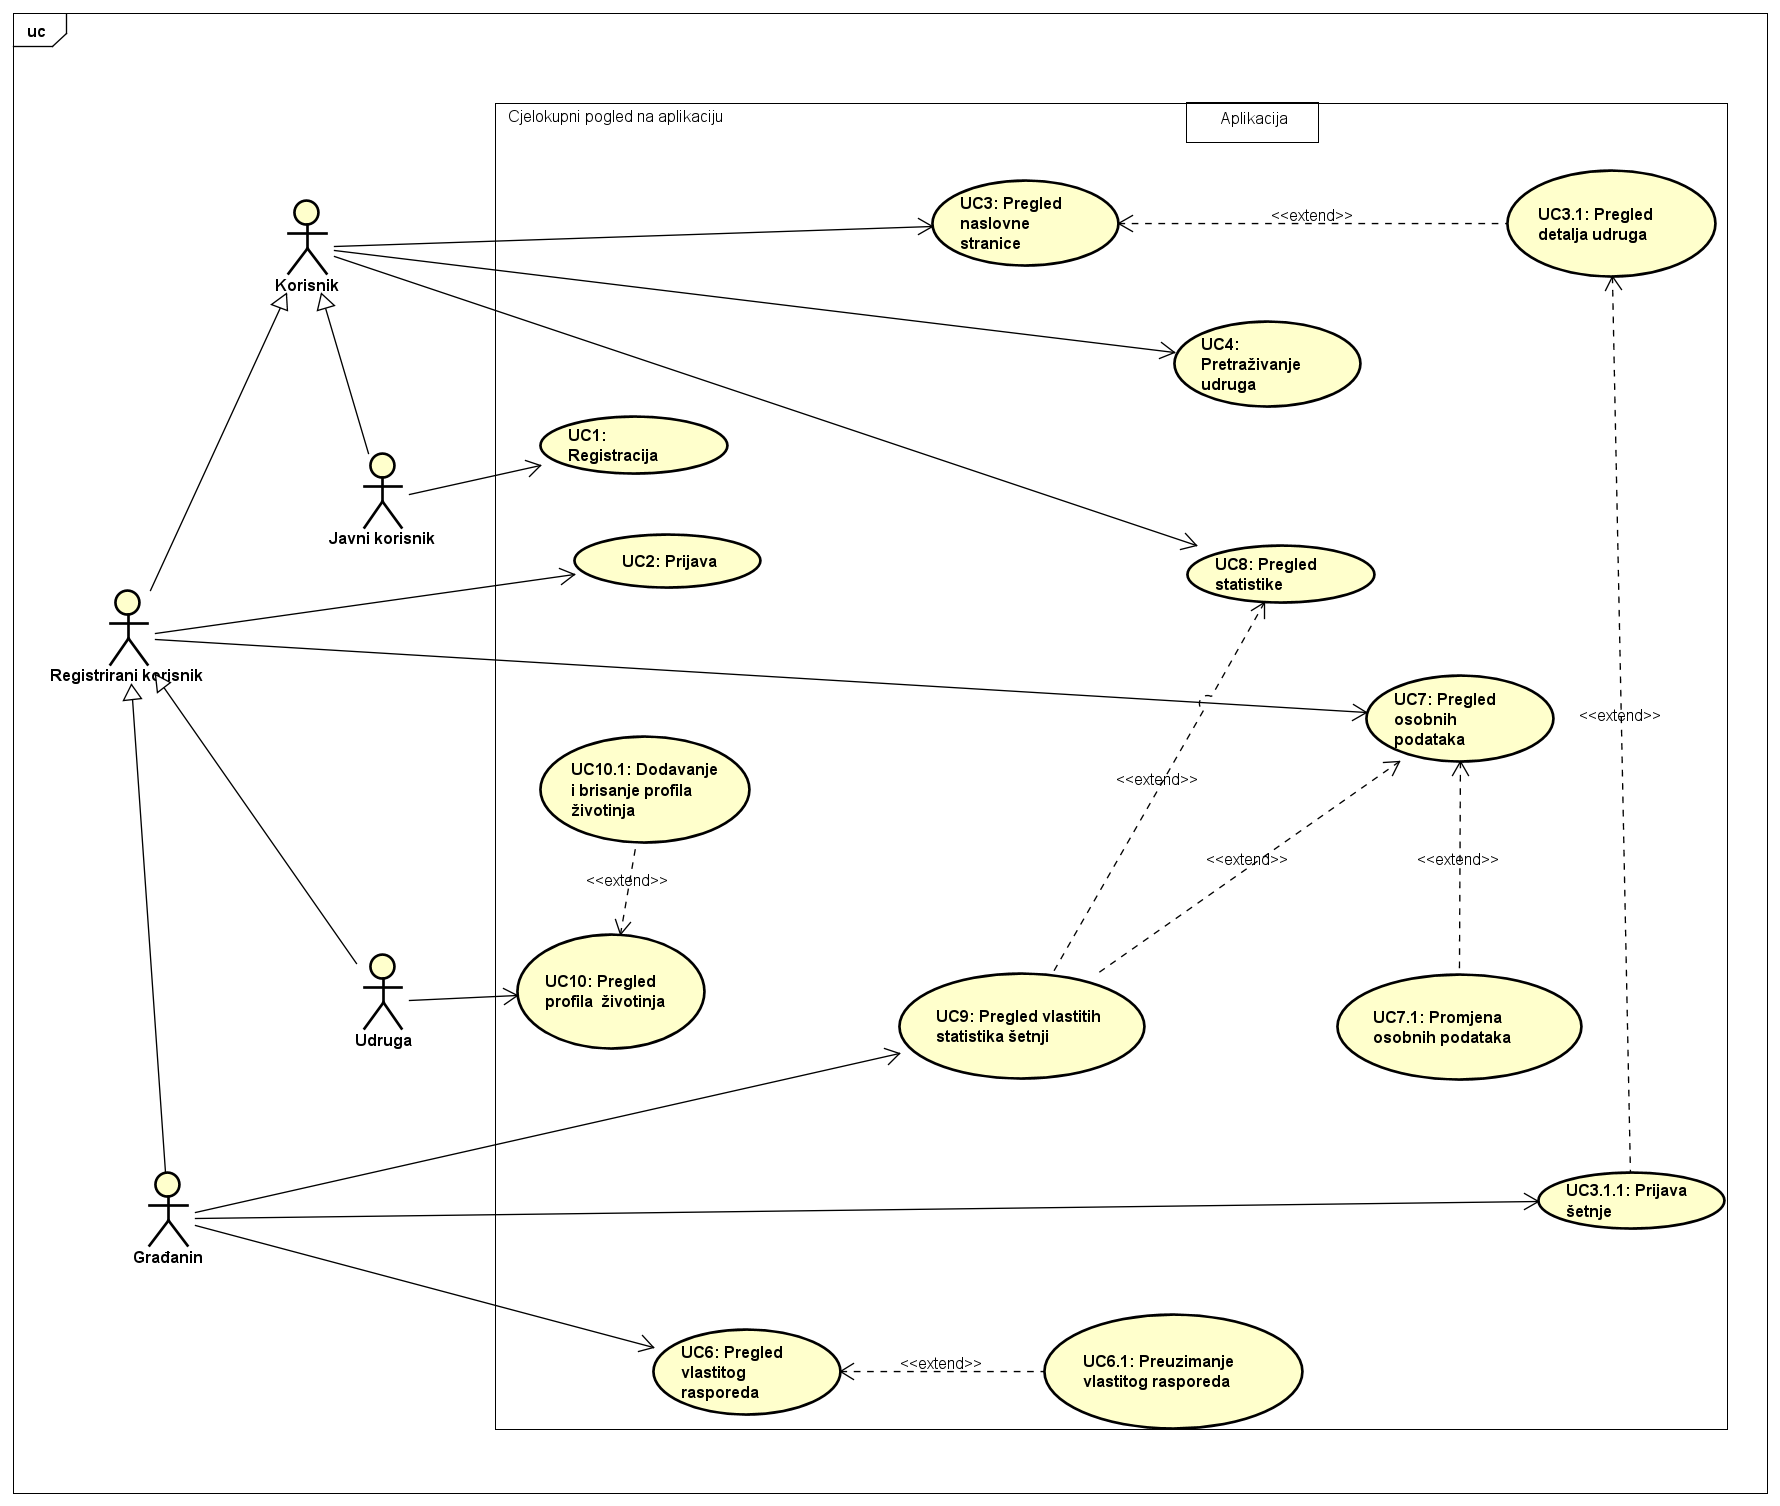
\includegraphics[width=\linewidth]{slike/UML.png}
						\centering
						\caption{Dijagram svih obrasca uporabe}
						\label{fig:uml}
					\end{figure}
					
				\eject		
				
			\subsection{Sekvencijski dijagrami}
				\noindent\textbf{Obrazac uporabe UC5 - Prijava šetnje}\\
				
				\noindent Građanin pregledom Udruge te odabirom željenog termina, šalje zahtjev za prikaz dostupnih životinja
				u terminu. Poslužitelj dohvaća sve slobodne životinje u odabranom terminu iz baze podataka, te ih 
				prikazuje. Ako je Građanin zadovoljan odabirom slobodnih životinja, odabire željeni oblik šetnje.
				Zatim se životinje filtriraju po odabranoj vrsti šetnje i prikazuju. Građanin odabire željene 
				životinje za termin. Kada je Građanin zadovoljan s odabirom, može poslati zahtjev za potvrdu 
				šetnje. Potvrdom šetnje se zauzima termin životinja te se prikazuje poruka "Šetnja prijavljena".
				
				\begin{figure}[H]
					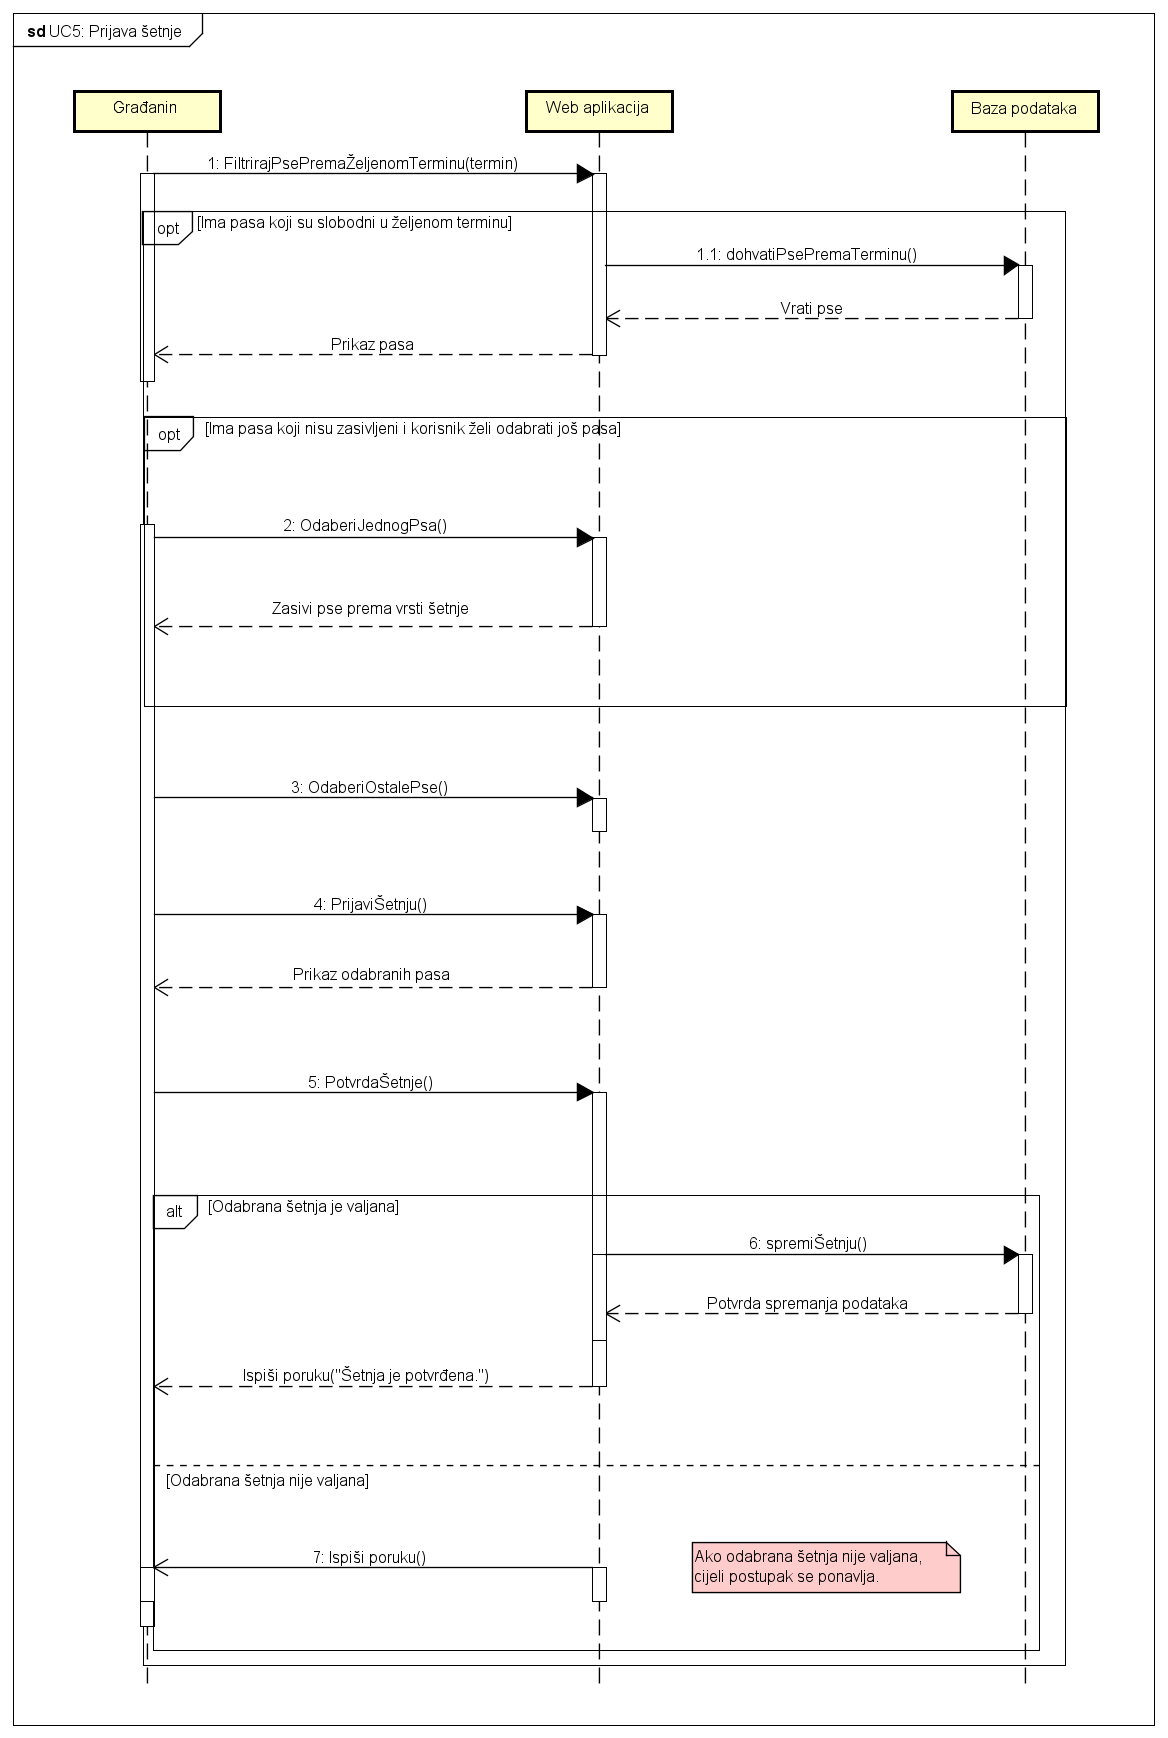
\includegraphics[width=\linewidth]{slike/SEK-5.png}
					\centering
					\caption{Sekvencijski dijagram za UC5}
					\label{fig:sek-5}
				\end{figure}
			
				\pagebreak
				\noindent\textbf{Obrazac uporabe UC6 i UC6.1 - Pregled i preuzimanje vlastitog rasporeda}\\
				
				\noindent Građanin šalje zahtjev za pregled vlastitog rasporeda. Poslužitelj dohvaća raspored 
				te mu ga prikazuje. Građanin je u mogućnosti odabirom opcije "Preuzmi vlasititi raspored" 
				zatražiti preuzimanje vlastitog raspored u PDF formatu.
				
				\begin{figure}[H]
					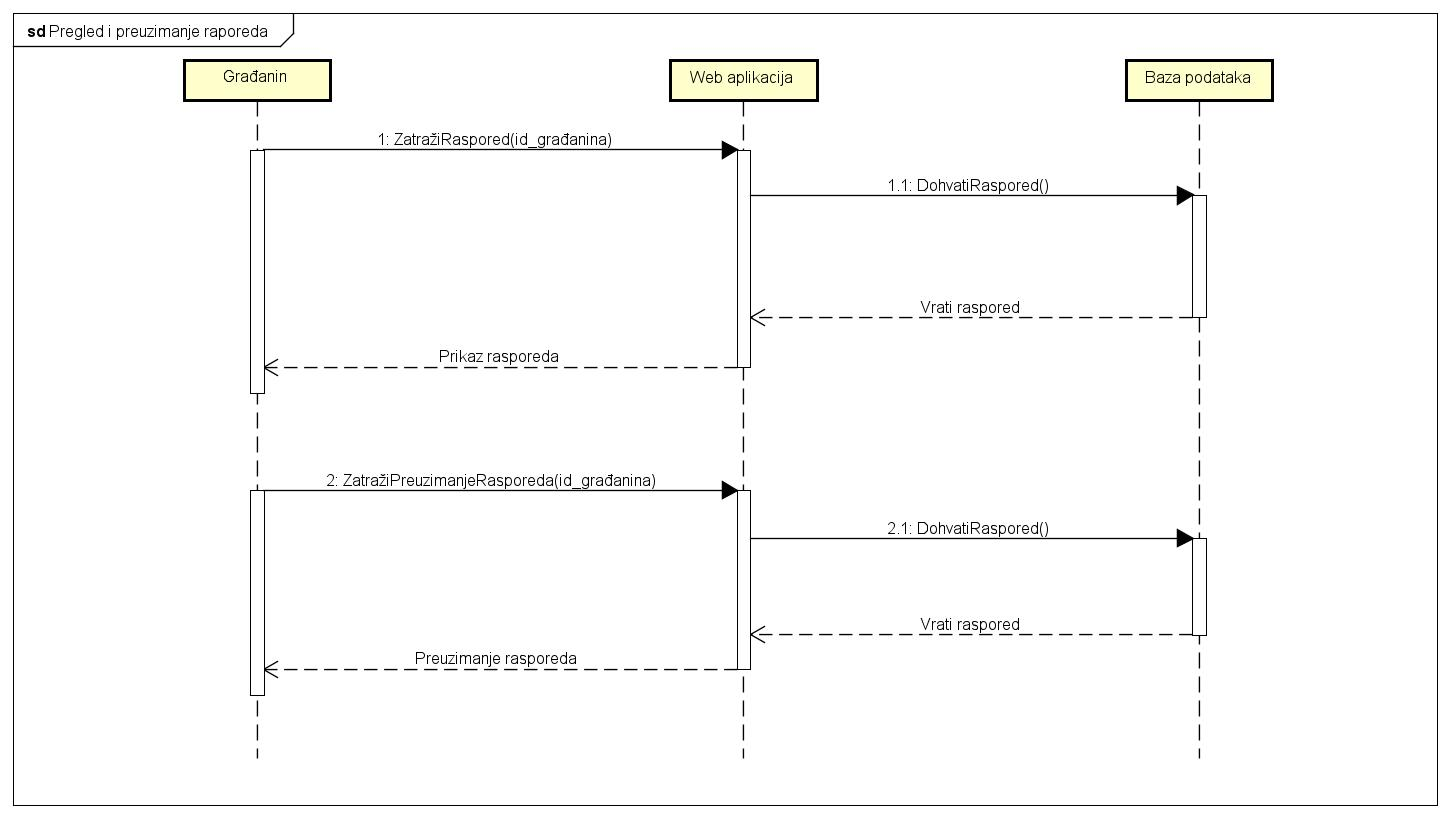
\includegraphics[width=\linewidth]{slike/SEK-6-6.1.jpg}
					\centering
					\caption{Sekvencijski dijagram za UC6 i UC6.1}
					\label{fig:sek-6-6.1}
				\end{figure}
				
				\eject
	
		\section{Ostali zahtjevi}
			 
			 
			 
			 \begin{packed_item}
			 	
			 	\item Sustav treba biti intuitivan i jednostavan za korištenje korisnicima koji prvi put koriste aplikaciju.
			 	\item Sustav mora omogućiti pristup i rad više korisnika istovremeno.
			 	\item Sustav treba biti implementiran kao web aplikacija i mora mu biti omogućen pristup iz javne mreže pomoću HTTPS protokola.
			 	\item Neregularne aktivnosti unutar sustava ne smiju narušiti njegov rad i daljnje normalno funkcioniranje.
			 	\item Sustav mora podržavati hrvatska slova (dijakritičke znakove).
			 	\item Baza podataka mora biti zaštićena, brza i otporna na moguće pogrešne zahtjeve.
			 	\item Dohvaćanje podataka iz baze ne smije trajati duže od nekoliko sekundi. 
			 	\item Sustav treba biti moguće nadograđivati, unaprijeđivati i razvijati bez narušavati postojećih funkcionalnosti.
			 	\item Prilikom prijave šetnje njezino trajanje mora biti zaokruženo na puni sat.
			 	\item Statistika prikazuje podatke stare do 30 dana.
			 	\item Datum mora biti u obliku dd-mm-yyyy.
			 	
			 \end{packed_item}


			 
			 
			 
	